\chapter{Use Case}
\section{Overall Objective}
The main goal of this application is to monitor energy usage to encourage smart decisions within 3D printer companies. This prevents both energy waste and the waste of materials used in printing. This would save money and resources in the long run, optimizing prints and reducing energy bills.

\section{Energy Consumption Monitoring and Sustainability Analytics}
As manufacturing facilities scale their 3D printer fleets, tracking and optimizing energy consumption becomes a critical operational requirement. \textbf{\textit{Eco3DPrint}} acts as an advanced telemetry pipeline, serializing real-time power measurements into SenML-compliant JSON payloads and transmitting them to a central database. The system's cloud backend aggregates this data to perform granular cost accounting and sustainability analysis. Through the frontend interface, operators can generate comprehensive daily, weekly, and monthly reports. Crucially, the system dichotomizes power consumption into "well-used" energy (attributed to successfully completed prints) and "wasted" energy (attributed to aborted or failed prints). This visibility enables facility managers to identify inefficient hardware, optimize print parameters to reduce failure rates, and accurately calculate the true energy overhead of their additive manufacturing processes.

\section{Predictive Maintenance and Automated Fault Detection}
In traditional 3D Printing Environments, mechanical failures such as layer shifting, print bed detachment, or nozzle clogging often go unnoticed until the print cycle is manually inspected. This results in significant material waste and prolonged equipment downtime. \textbf{\textit{Eco3DPrint}} addresses this through autonomous edge intelligence. By continuously sampling multi-axis vibration and power draw via attached sensor nodes (e.g., nRF52840 dongles equipped with accelerometers and power monitors), the system captures the high-frequency physical state of the machine. An embedded Machine Learning model analyzes these localized time-series windows to detect anomalies in real time. Upon identifying a critical failure signature for consecutive cycles, the edge node autonomously aborts the printing process. This rapid, localized decision-making minimizes material waste and prevents potential hardware damage without relying on constant cloud connectivity or human supervision.

\section{Remote Fleet Orchestration and Job Dispatching}
Managing a distributed array of additive manufacturing nodes requires a centralized, responsive command interface. \textbf{\textit{Eco3DPrint}} provides a full-duplex, asynchronous control plane that allows human operators to monitor and manipulate the entire fleet from a single desktop application. Through the graphical dashboard, users receive immediate, color-coded situational awareness regarding the availability and operational status of each node. Furthermore, the system streamlines the production workflow by enabling remote job dispatching. Operators can seamlessly query the backend for available STL models and queue them for specific printers. The backend orchestrates the reliable delivery of these large binary assets using CoAP block-wise transfer, overcoming the memory constraints of the physical edge nodes and ensuring that production can be scaled efficiently without physical intervention at each machine. 

\section{Application Working}
\begin{figure}[H]
	\centering
	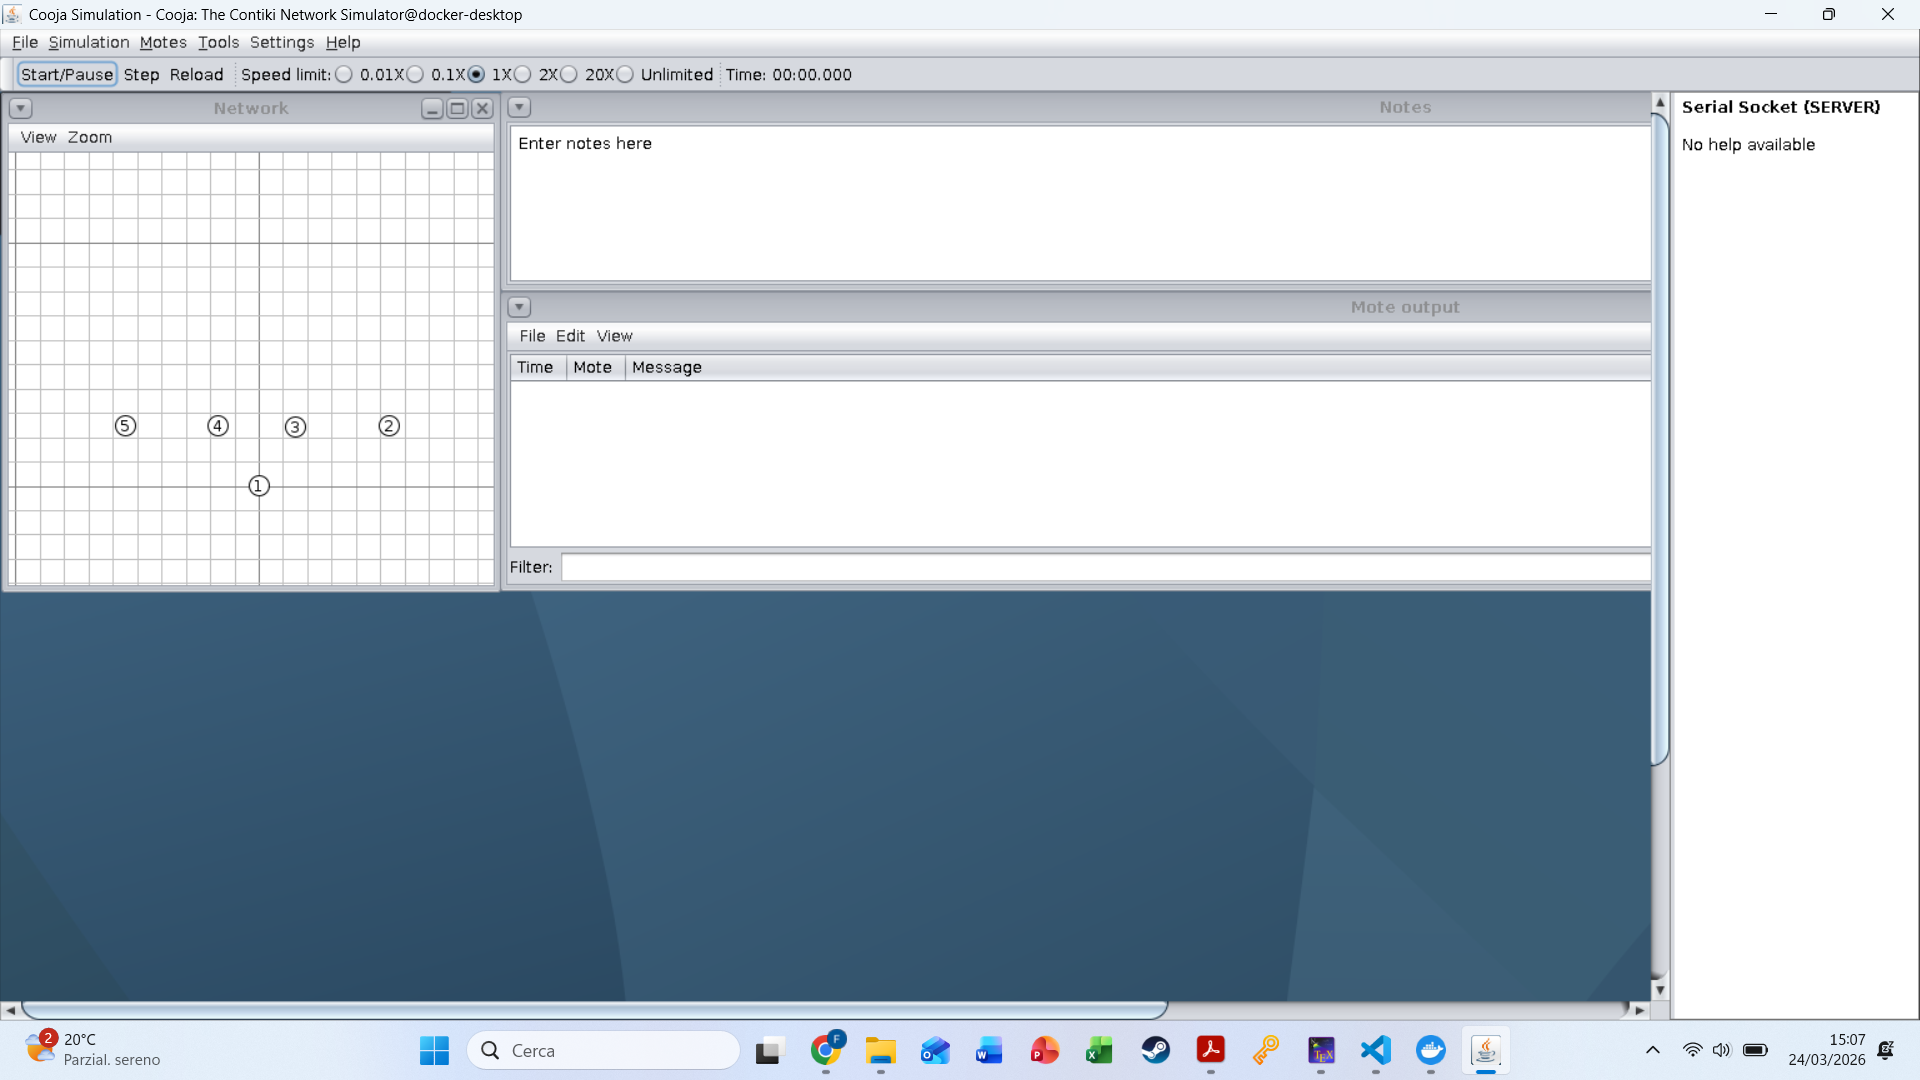
\includegraphics[width=0.675\textwidth]{img/Screenshot_1.png}
	\caption{Starting Cooja}
	\label{fig:Screenshot-1}
\end{figure}

\begin{figure}[H]
	\centering
	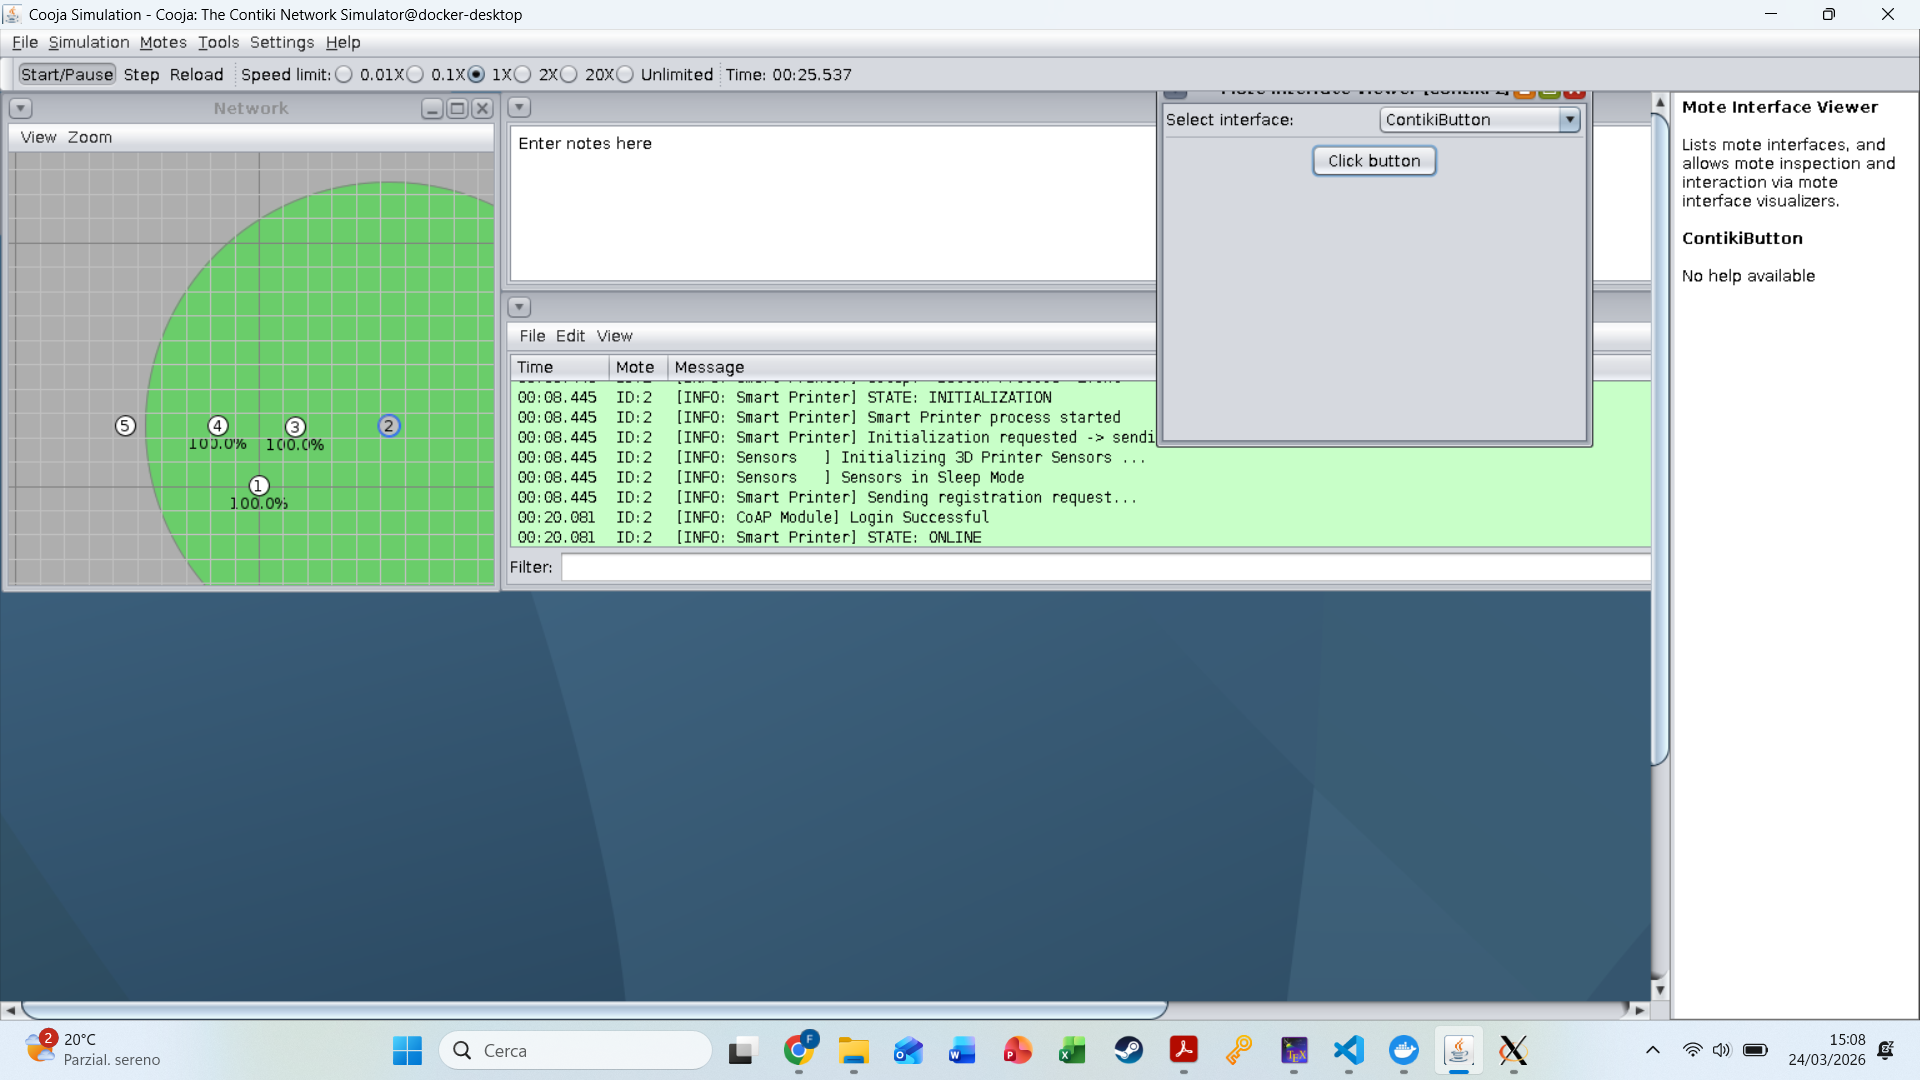
\includegraphics[width=0.675\textwidth]{img/Screenshot_2.png}
	\caption{Click button and start the Mote}
	\label{fig:Screenshot-2}
\end{figure}

\newpage

\begin{figure}[H]
	\centering
	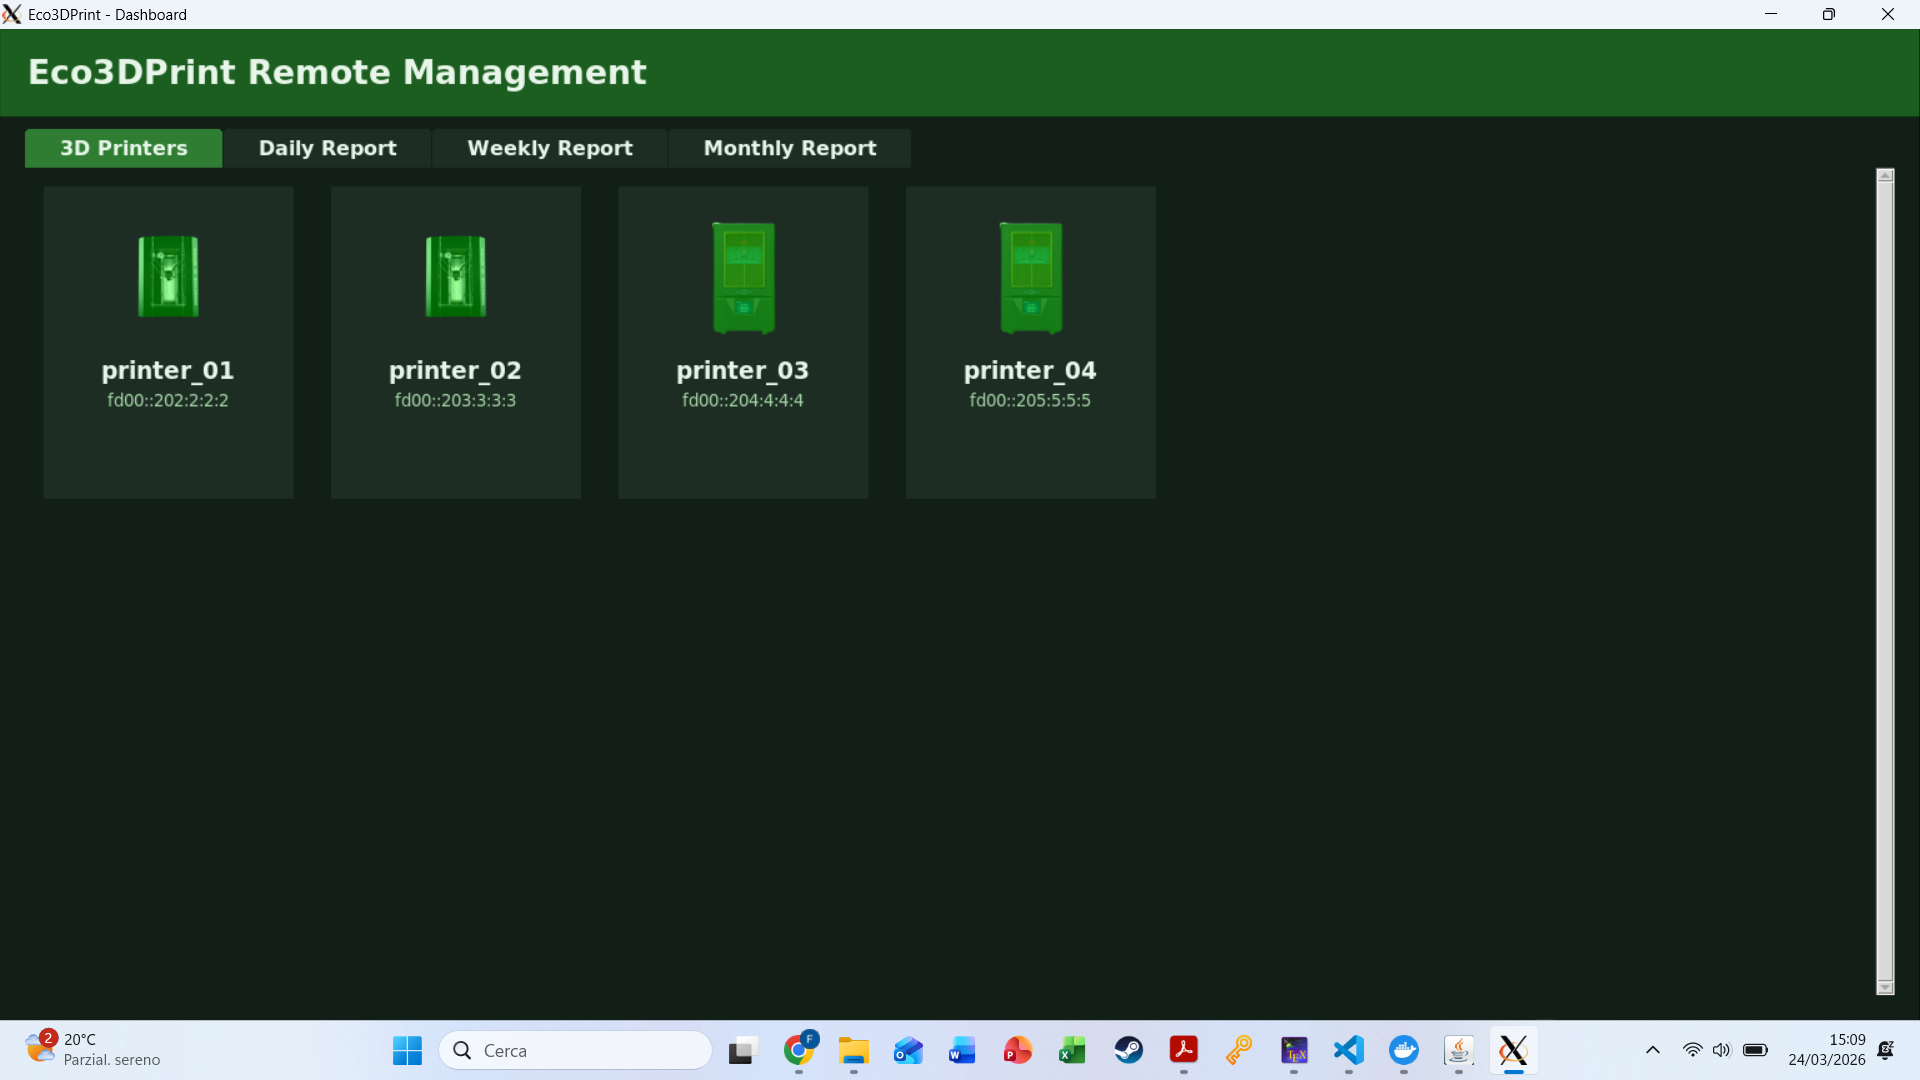
\includegraphics[width=0.675\textwidth]{img/Screenshot_3.png}
	\caption{User Application Printer Screen}
	\label{fig:Screenshot-3}
\end{figure}

\begin{figure}[H]
	\centering
	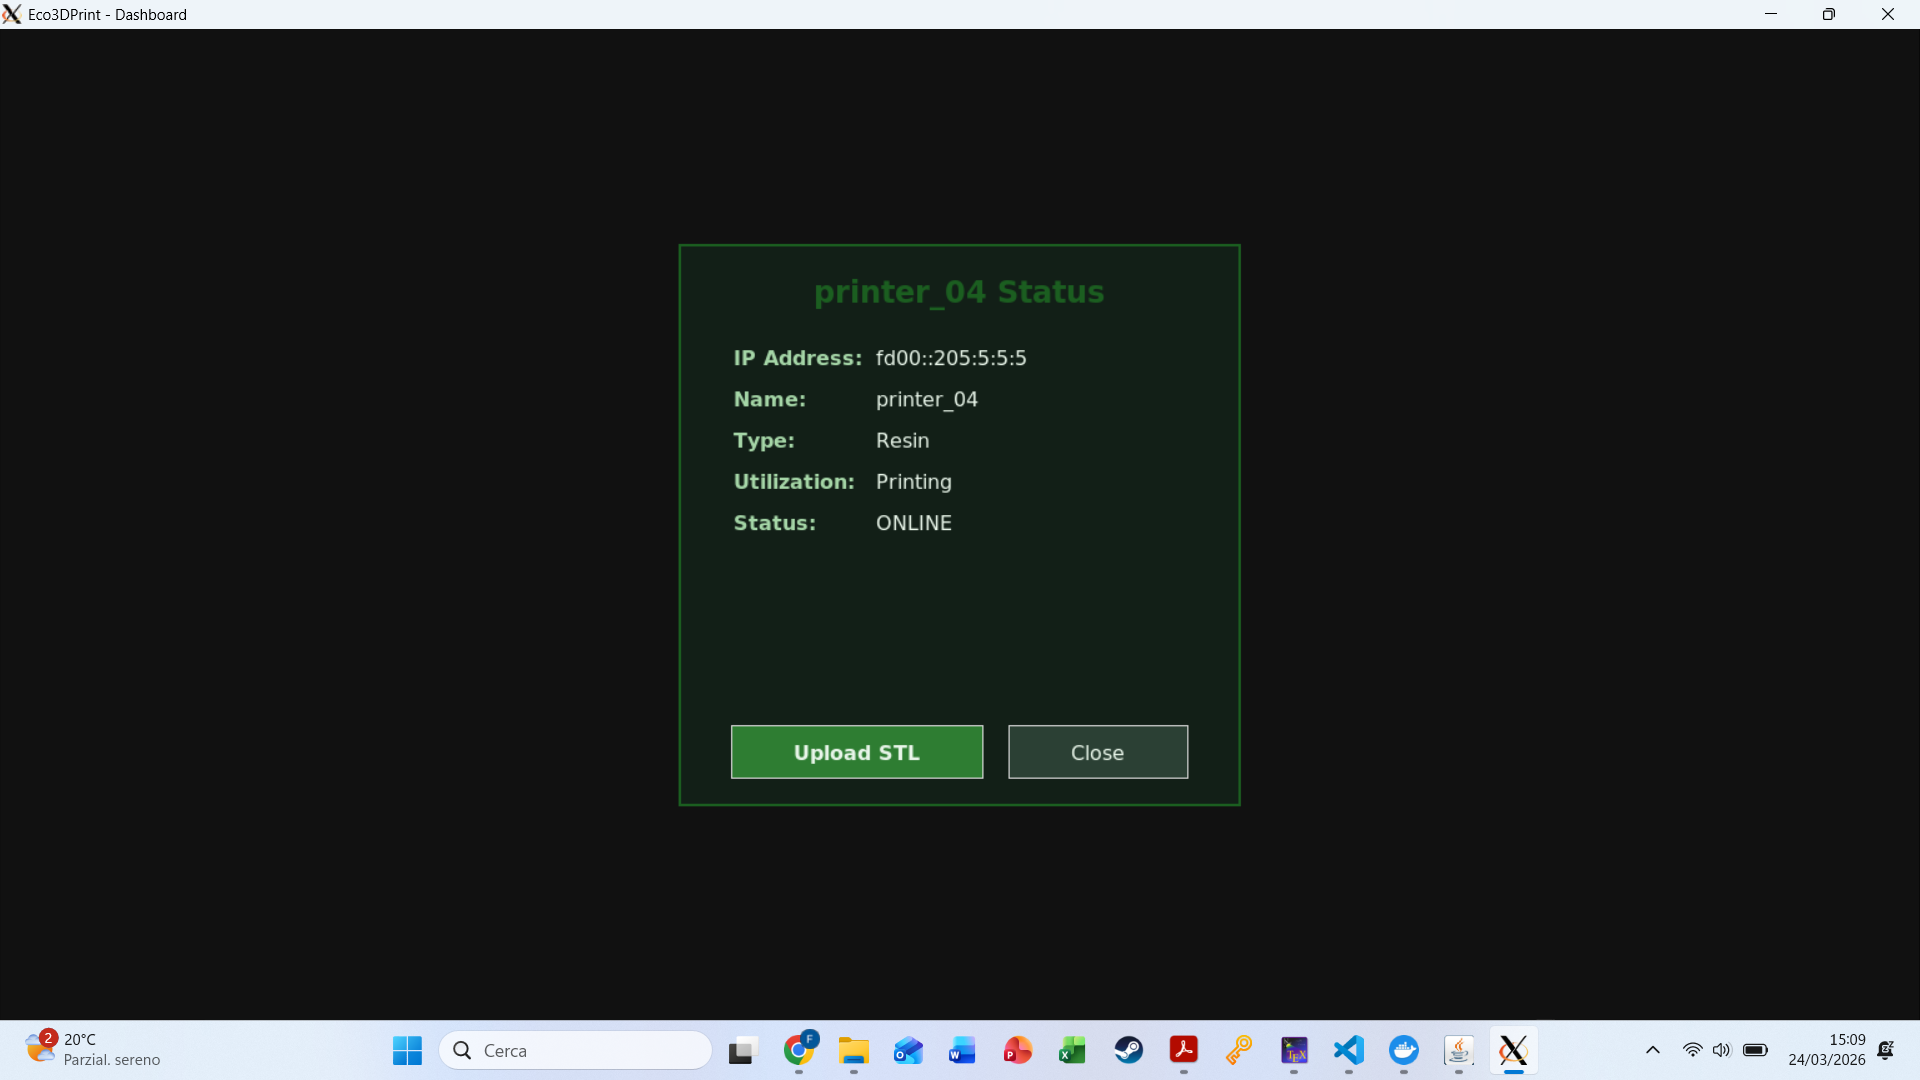
\includegraphics[width=0.675\textwidth]{img/Screenshot_4.png}
	\caption{Upload STL}
	\label{fig:Screenshot-4}
\end{figure}

\begin{figure}[H]
	\centering
	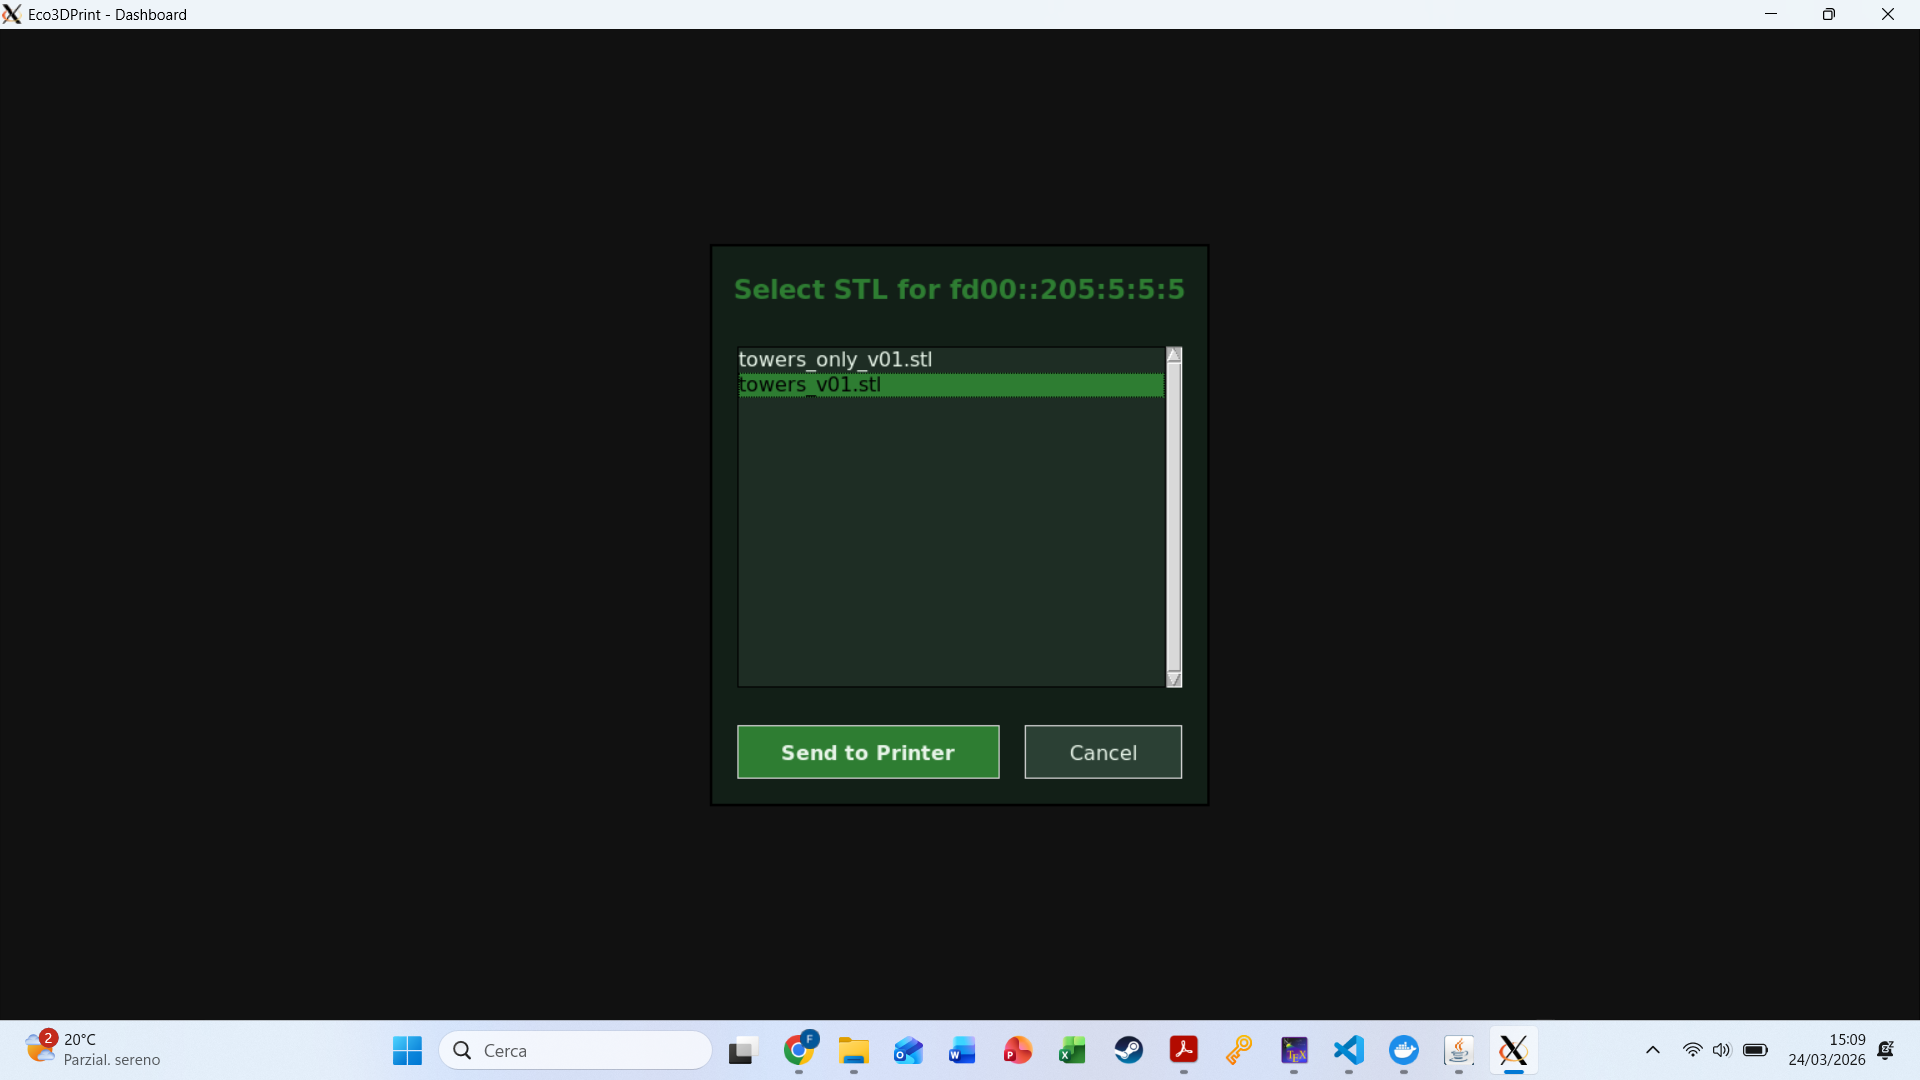
\includegraphics[width=0.675\textwidth]{img/Screenshot_5.png}
	\caption{Send STL}
	\label{fig:Screenshot-5}
\end{figure}

\newpage

\begin{figure}[H]
	\centering
	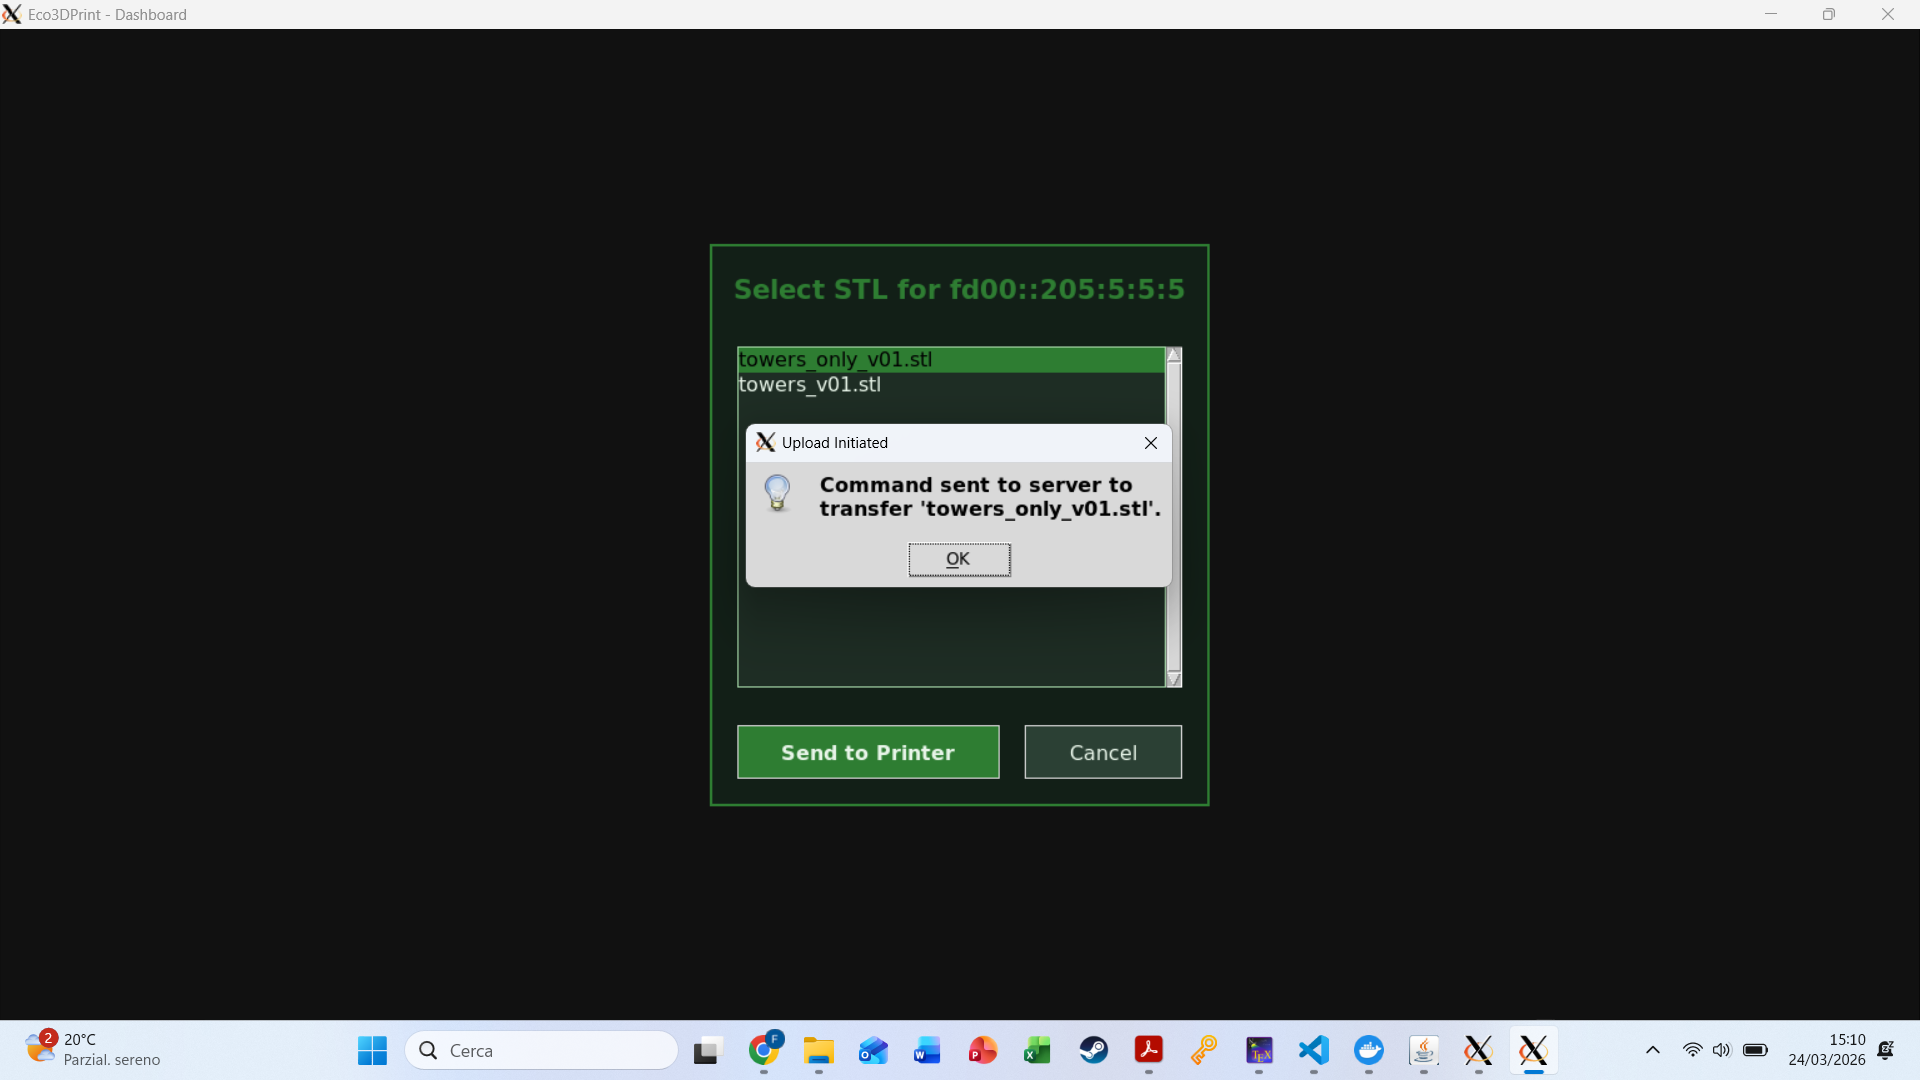
\includegraphics[width=0.675\textwidth]{img/Screenshot_6.png}
	\caption{STL Transfered and Start Printing}
	\label{fig:Screenshot-6}
\end{figure}

\begin{figure}[H]
	\centering
	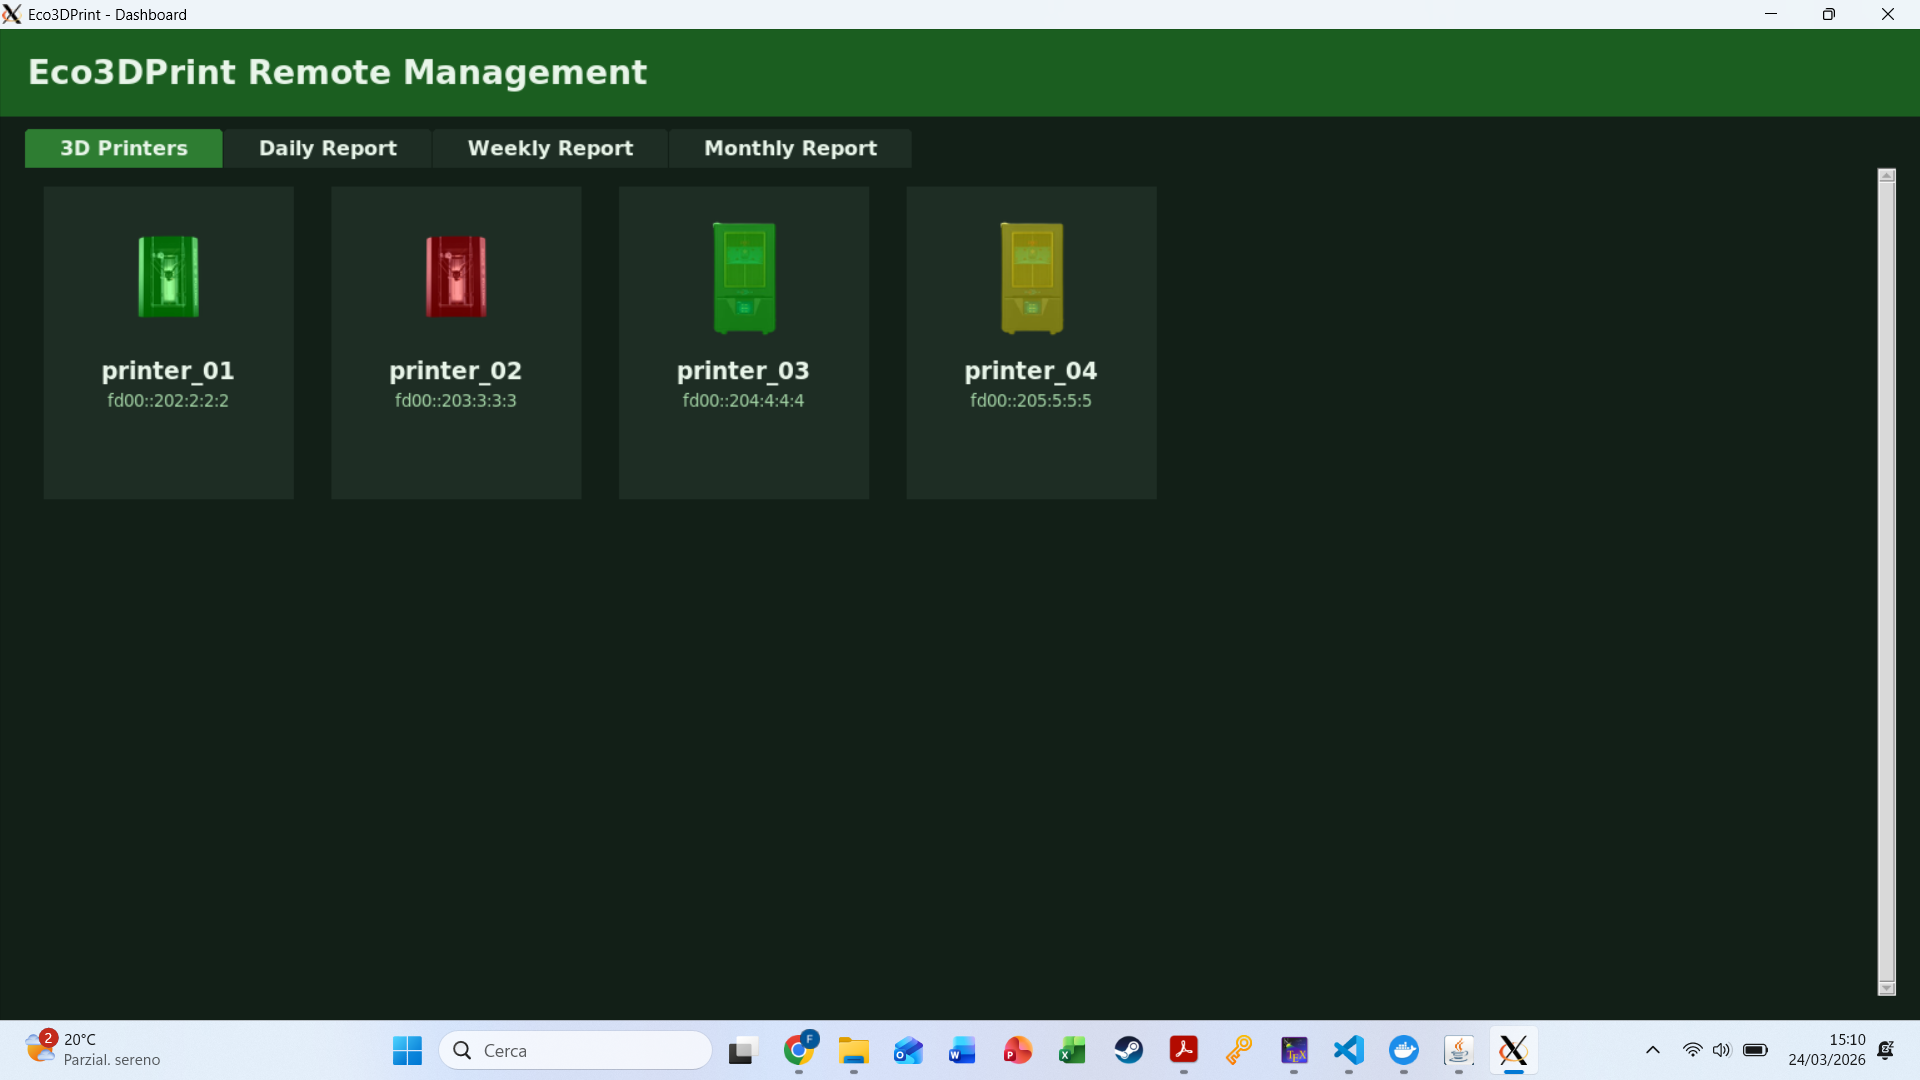
\includegraphics[width=0.675\textwidth]{img/Screenshot_7.png}
	\caption{Printer 1 Online, Printer 2 Offline, Printer 3 Online, and Printer 4 Printing}
	\label{fig:Screenshot-7}
\end{figure}

\begin{figure}[H]
	\centering
	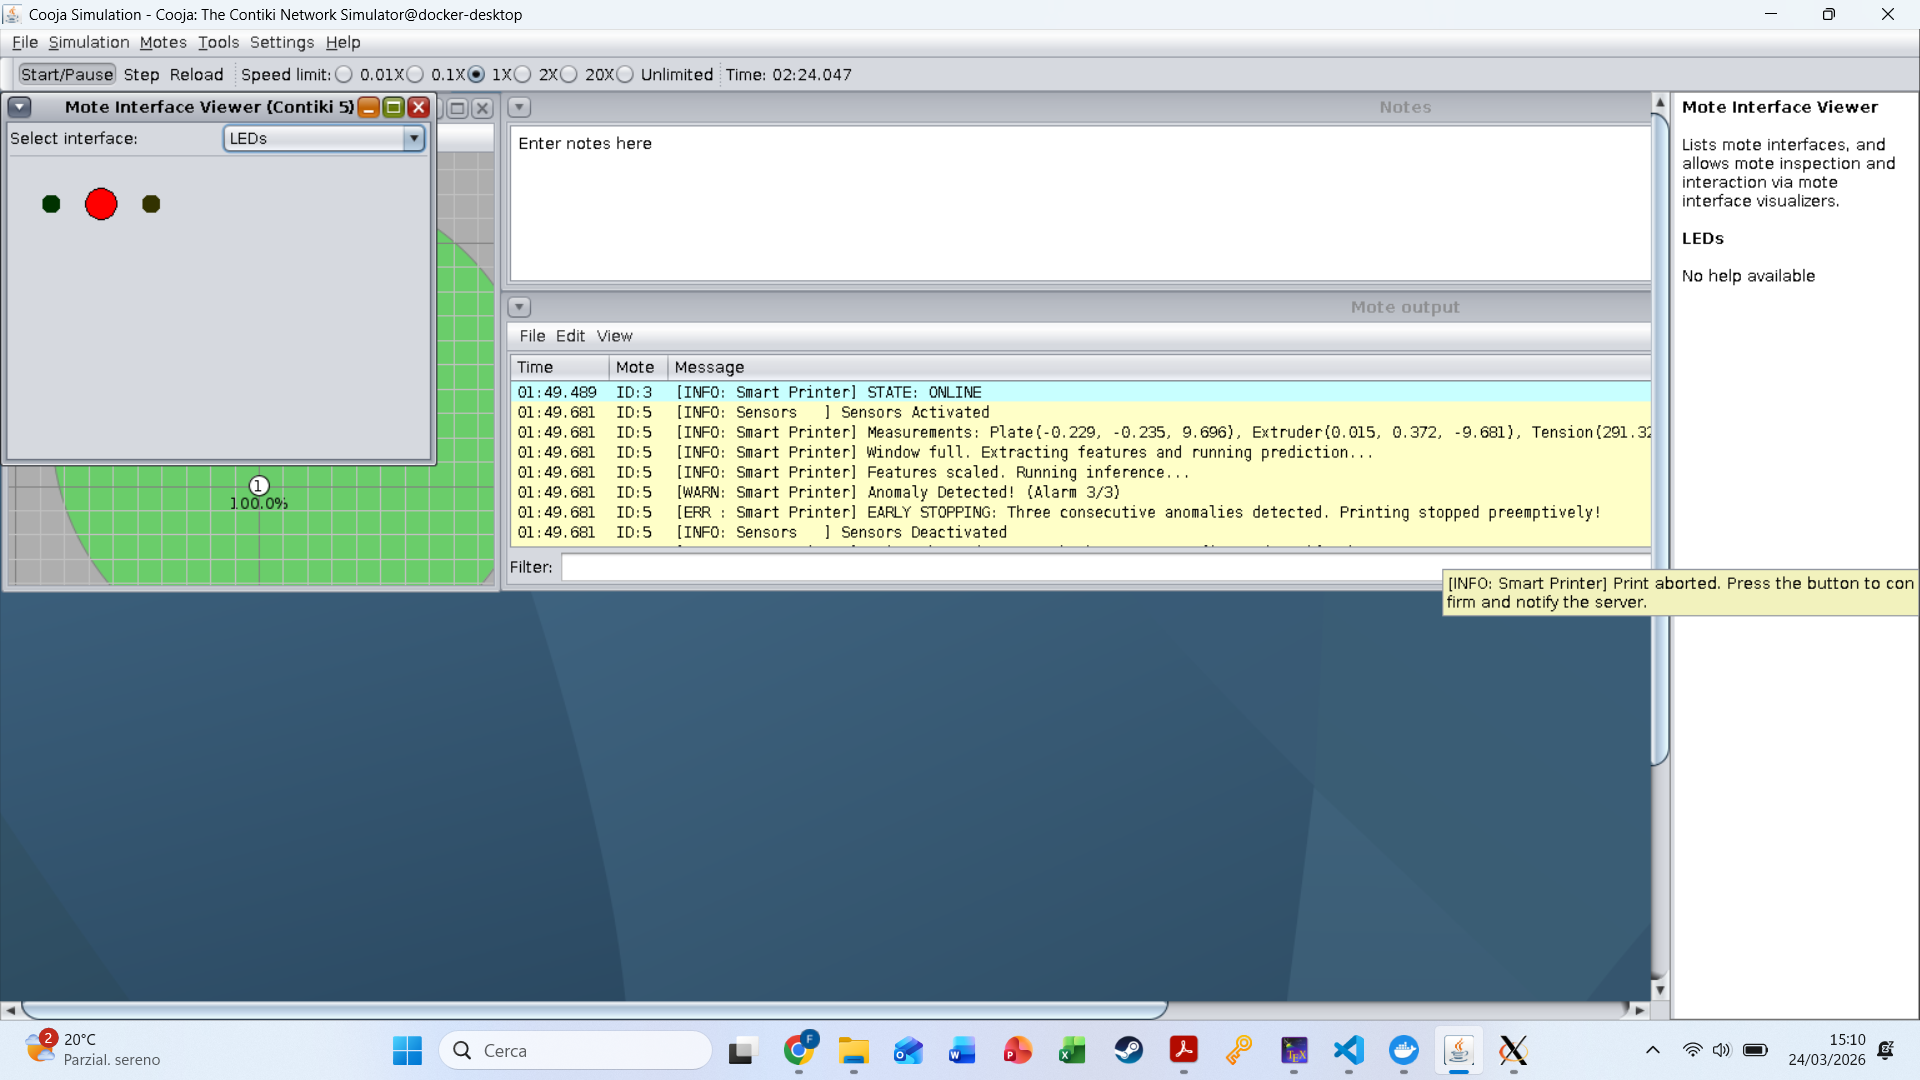
\includegraphics[width=0.675\textwidth]{img/Screenshot_8.png}
	\caption{Printer Blocked by Machine Learning Model}
	\label{fig:Screenshot-8}
\end{figure}

\newpage

\begin{figure}[H]
	\centering
	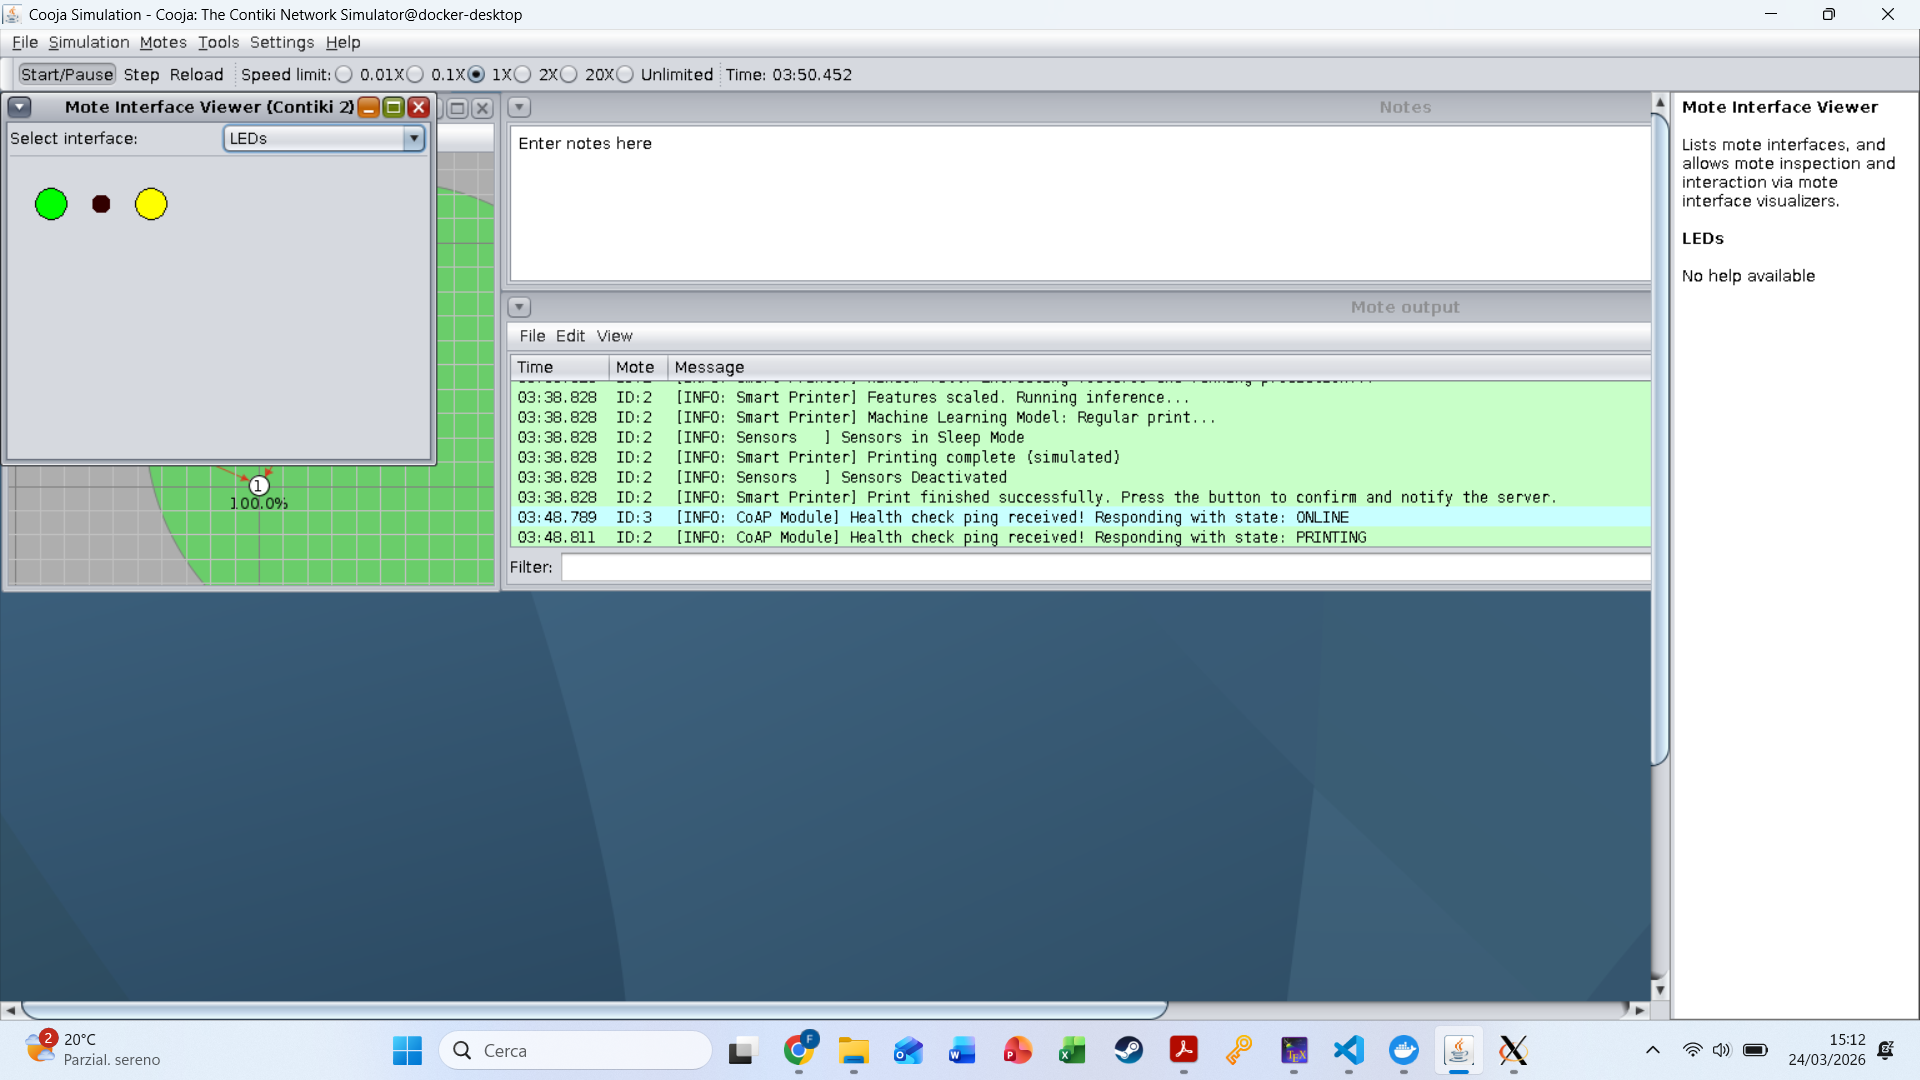
\includegraphics[width=0.675\textwidth]{img/Screenshot_9.png}
	\caption{Succesfull Print}
	\label{fig:Screenshot-9}
\end{figure}

\begin{figure}[H]
	\centering
	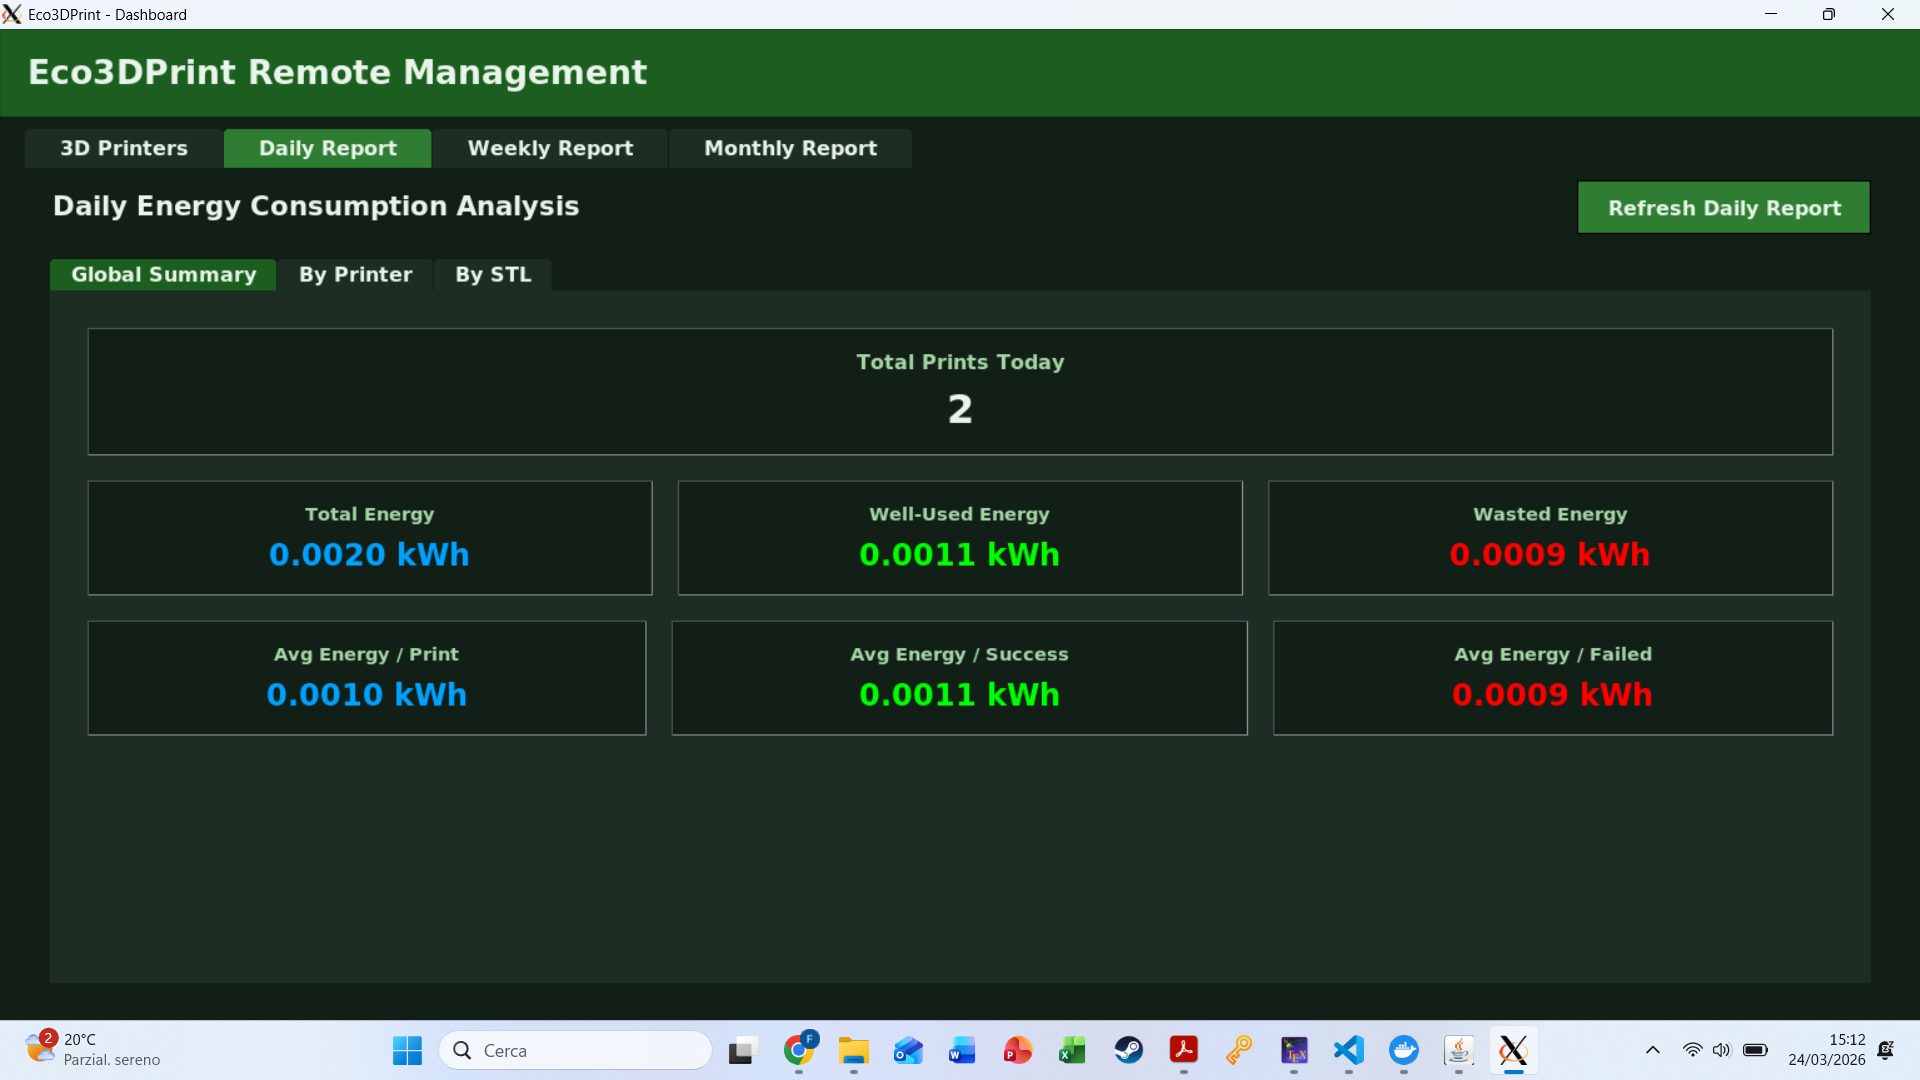
\includegraphics[width=0.675\textwidth]{img/Screenshot_10.png}
	\caption{Daily Report}
	\label{fig:Screenshot-10}
\end{figure}

\begin{figure}[H]
	\centering
	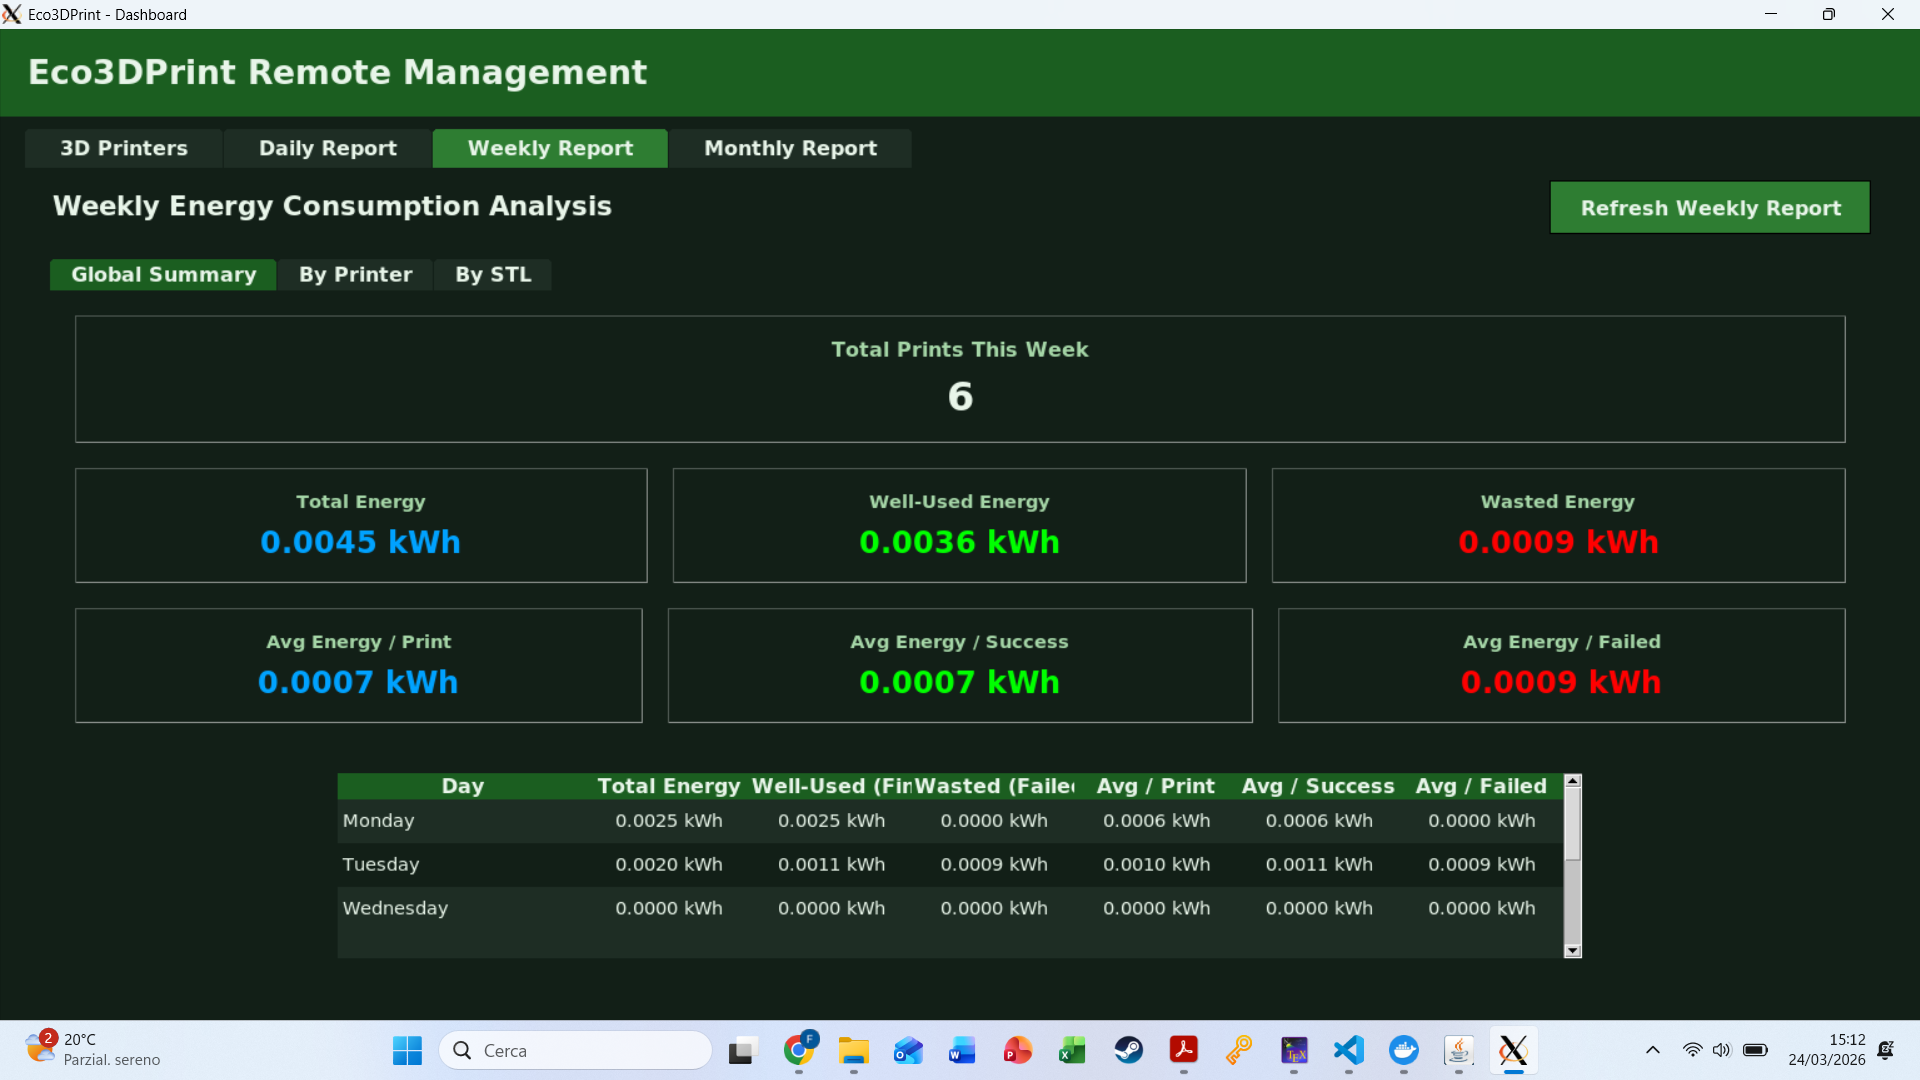
\includegraphics[width=0.675\textwidth]{img/Screenshot_11.png}
	\caption{Weekly Report}
	\label{fig:Screenshot-11}
\end{figure}

\newpage

\begin{figure}[H]
	\centering
	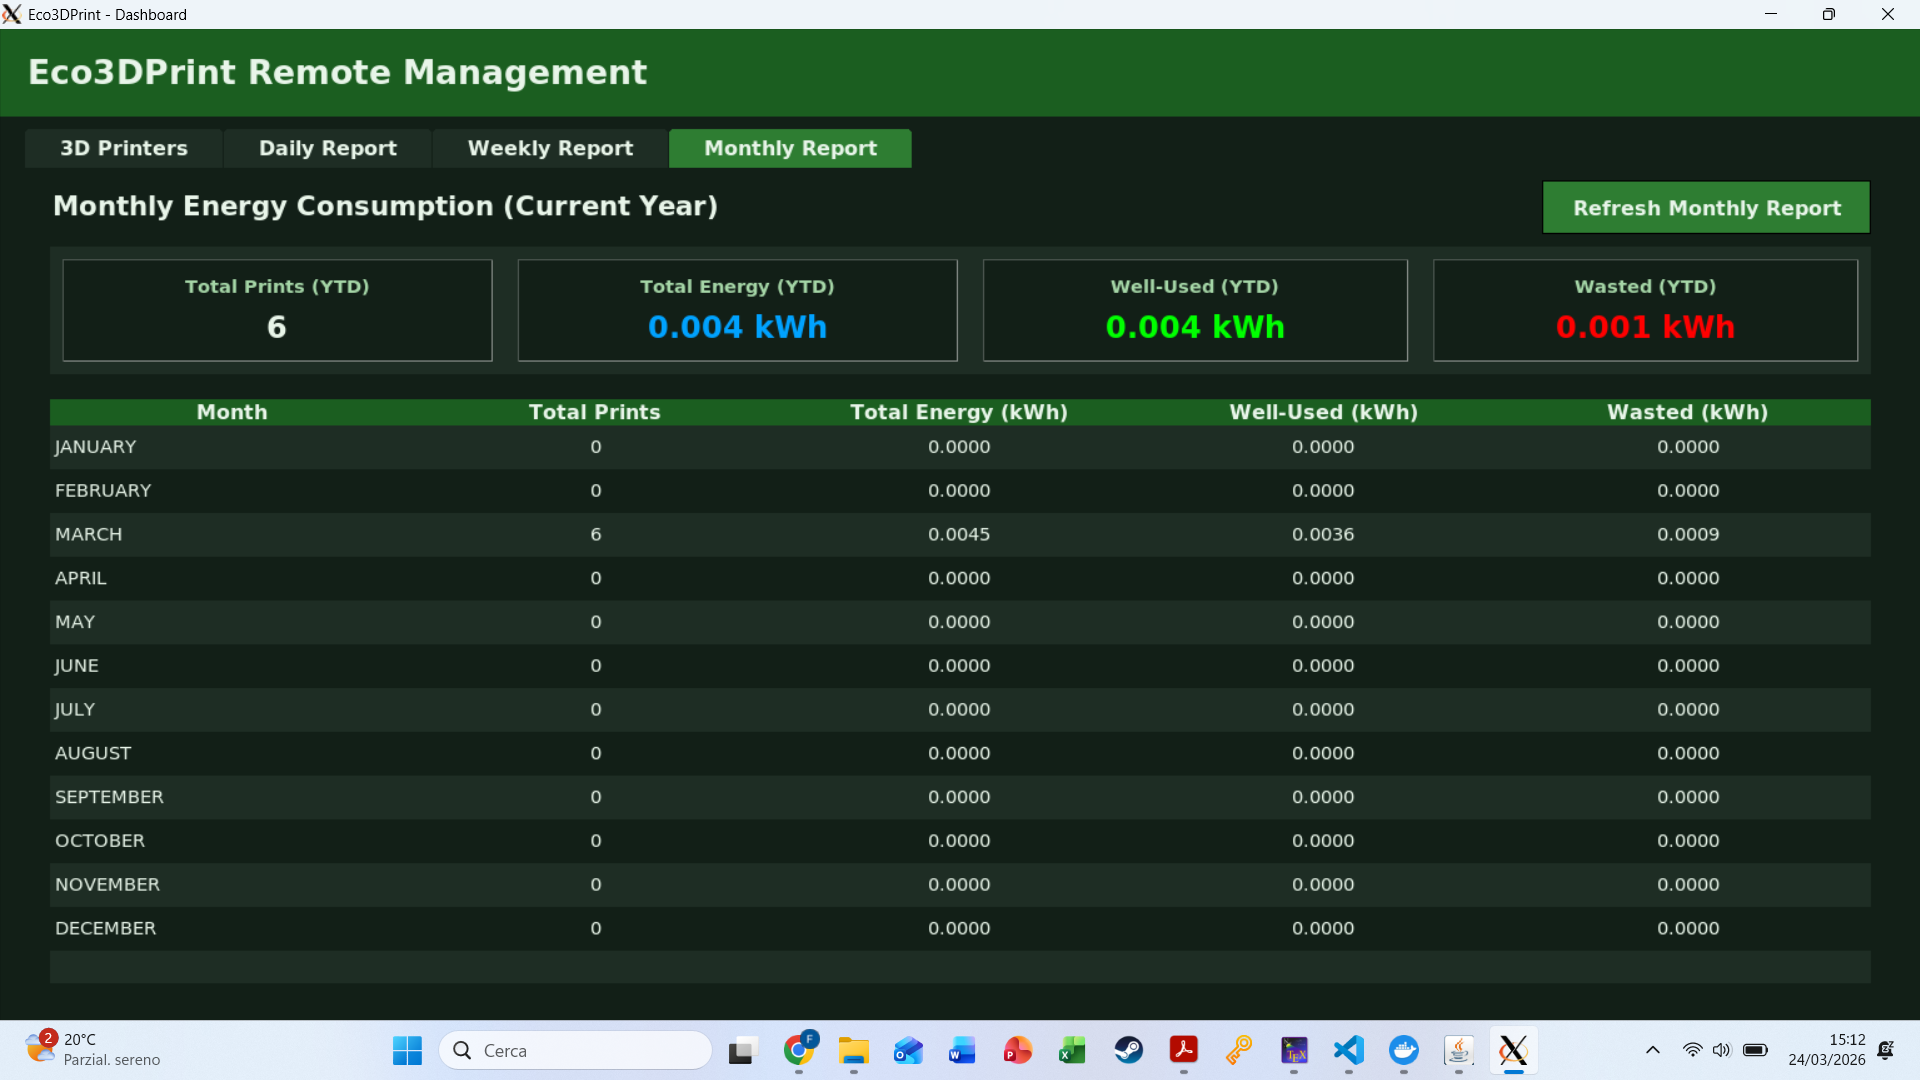
\includegraphics[width=0.9\textwidth]{img/Screenshot_12.png}
	\caption{Monthly Report}
	\label{fig:Screenshot-12}
\end{figure}






